% This template was created by Chris Hoofnagle for 
% the Berkeley Center for Law & Technology. If you 
% work for UCB, you are welcome to use it.


\documentclass[letterpaper,12pt,twoside]{report}

% This is a "report" document class, which means that it has chapters
% and formatting like a book, but fundamentally is a design for
% one-sided printing. There are many options to change the underlying
% design---you can change the font, paper size, etc with these 
% options below. Just put the options in the braces of 
% \documentclass

% Documentclass: Report Options: a4paper, a5paper, b5paper, letterpaper, legalpaper, landscape, 11pt, 12pt, twoside, twocolumn, notitlepage, openright, draft, fleqn, leqno, openbib

%\usepackage[utf8]{inputenc}
\usepackage{booktabs}
\usepackage{graphicx}
% \usepackage{lipsum} % generates lorem ipsum filler text
\usepackage[most,many,skins,breakable]{tcolorbox}
\usepackage{xcolor}
\usepackage{tikz}
\usepackage{tikzpagenodes}
\tcbuselibrary{skins,breakable,xparse}
\usepackage{fancyhdr}
\usepackage[default,scale=0.95]{opensans}
\usepackage[hidelinks]{hyperref} % the hidelinks option prevents those terrible boxes from appearing in your print pdf
% \usepackage[backend=biber,language=american,style=verbose]{biblatex}
% \usepackage[citestyle=numeric, bibstyle=authortitle, sorting=anyt]{biblatex}
% \addbibresource{bibliography.bib}
\usepackage[natbibapa]{apacite}
\usepackage{natbib}
% \usepackage[numbers]{natbib}
% \usepackage{cite}
\usepackage[headheight=15pt,hmarginratio=1:1]{geometry}

%%%%%%%%%%%%%%%%%%%%%%%%
%
% Berkeley Colors - Global (changing these will alter the whole
% document)
%
%%%%%%%%%%%%%%%%%%%%%%%%

% Deep blue and gold
\definecolor{berkeleyblue}{HTML}{003262}
\definecolor{berkeleygold}{HTML}{FDB515}
% Light blue and gold
\definecolor{founderblue}{HTML}{3B7EA1}
\definecolor{founderyellow}{HTML}{C4820E}

%%%%%%%%%%%%%%%%%%%%%%%%
%
% Headings
%
%%%%%%%%%%%%%%%%%%%%%%%%

\fancyhf{}
% If you'd like, you can put the title of the report in the header
% Just erase title of report if not

\small\fancyhead[R] {\color{founderblue}Identify Airport Connections Based on Delay Patterns~ \thepage}
% This adds the line below the header. You can make it thicker or thinner by editing the 0.4 value
\renewcommand{\headrulewidth}{0.4pt}
% This template only uses a header because a document with footnotes
% looks strange with a footer. But if you want a footer, just 
% uncomment the lines below
%\small\fancyfoot[R] {\color{founderblue}Title of Report ~ \thepage}
%\renewcommand{\footrulewidth}{0.0pt}

%%%%%%%%%%%%%%%%%%%%%%%%
%
% Customizing Fonts & Title Formats - Global
%
%%%%%%%%%%%%%%%%%%%%%%%%

% This section specifies the fonts and their sizes and 
% colors for the headings. Notice that the package gives
% you serif headings and san serif body text.

\usepackage{titlesec}
\usepackage{fontspec}

% The headings are Berkeley's Old Style Fonts!
% I don't like the new fonts, which are licensed from
% Adobe --- why would you do that?

\newfontfamily\headingfont{UCBerkeleyOS.otf}[
BoldFont = UCBerkeleyOSBold.otf,
ItalicFont = UCBerkeleyOSItalic.otf,
BoldItalicFont = UCBerkeleyOSBoldItalic.otf]

% This controls the chapter headings

\titleformat{\chapter}{\fontsize{30}{60}\headingfont}{\color{founderblue}\thechapter\fontsize{90}{60}}{10pt}{\thispagestyle{empty}\color{founderblue}\Huge\bfseries}

% This controls the section and subsection headings in the chapters
% Notice that the headings in the chapter are numbered, e.g.
% 1.1 A Lesson in Latin. If you don't want section numbering,
% remove \thesection and/or \thesubsection

\titleformat{\section}{\Large\headingfont}{}{0pt}{\color{founderblue}{\thesection} \ }[{\titlerule[0.8pt]}]

\titleformat{\subsection}{\large\headingfont}{}{0pt}{\color{founderblue}{\thesubsection} \ }[{\titlerule[0.8pt]}]

% This customizes the sections in the executive summary so that they
% will not be numbered.

\titleformat{name=\section,numberless}
{\Large\headingfont}{}{-4pt}{\color{founderblue} \ }[{\titlerule[0.8pt]}]

\titleformat{name=\subsection,numberless}
{\large\headingfont}{}{-4pt}{\color{founderblue} \ }[{\titlerule[0.8pt]}]

%%%%%%%%%%%%%%%%%%%%%%%%
%
% Sidebar Environment: mdframed
%
%%%%%%%%%%%%%%%%%%%%%%%

% \usepackage{amstext}
\usepackage{amsmath,amsfonts,amssymb,amsthm}
\usepackage{mathtools}
\usepackage[framemethod=TikZ]{mdframed}


\mdfdefinestyle{custom}{frametitle={\colorbox{berkeleygold}{\space You must specify a title for your box \space}},
     frametitlefont=\textbf,
     backgroundcolor=founderblue!20,
     linecolor=founderblue!70,
     innertopmargin=10pt,
     frametitleaboveskip=-\ht\strutbox,
     skipabove=\topskip,
     skipbelow=\topskip}




%\newenvironment{sidebar}[1]
% \mdfsetup{%
% % Replace berkeleygold with white if you'd like
%     frametitle={\colorbox{berkeleygold}{\space#1\space}},
%     frametitlefont=\textbf,
%     backgroundcolor=founderblue!20,
%     linecolor=founderblue!70,
%     innertopmargin=10pt,
%     frametitleaboveskip=-\ht\strutbox,
% %    frametitlealignment=\left,
%     skipabove=\topskip,
%     skipbelow=\topskip
%     }%
%   \begin{mdframed}%
%   }
%   {\end{mdframed}}

%%%%%%%%%%%%%%%%%%%%%%%%
%
% Sidebars with tcolorbox -- Mybox
%
%%%%%%%%%%%%%%%%%%%%%%%

\newtcolorbox{mybox}[2][]{enhanced, interior hidden, 
coltitle=black, fonttitle=\bfseries\headingfont\large,
attach boxed title to top left={yshift=-2.5mm},
boxed title style={empty, size=small, top=1mm, bottom=2pt},
%boxed title=0.5\linewidth,
frame code={
\path (title.east|-frame.north) coordinate (aux);
\path[draw=founderblue, fill=founderblue!20, line width=0.5mm, rounded corners]
(frame.west) |- ([xshift=-2.5mm]title.north east) to[out=0, in=180] ([xshift=7.5mm]aux)-|(frame.east)|-(frame.south)-|cycle;  
},
title={#2},#1}

%%%%%%%%%%%%%%%%%%%%%%%%
%
% General Guidance
%
%%%%%%%%%%%%%%%%%%%%%%%

%\flushbottom

%The \flushbottom declaration makes all text pages the same height, adding extra vertical space when necessary to fill out the page.

%\onecolumn
%The \onecolumn declaration starts a new page and produces single-column output.

%\raggedbottom
%The \raggedbottom declaration makes all pages the height of the text on that page. No extra vertical space is added.

%\twocolumn
%The \twocolumn declaration starts a new page and produces two-column output.

%%%%%%%%%%%%%%%%%%%%%%%%
%
% Document Content Starts Here
%
%%%%%%%%%%%%%%%%%%%%%%%


\title{Understand Airport Operation Delays: A Graph Clustering Approach}

\begin{document}

% The title page appearance is controlled by a separate file named titlepage.tex
\addcontentsline{toc}{chapter}{Abstract}
\begin{titlepage}
\pagecolor{founderblue}
       \vspace*{1cm}


% This controls the title
% You can reposition this element by editing the numeric
% values in \node (1,1). The first value controls the 
% horizontal placement, the second the vertical.

\tikz[overlay, remember picture] \node at (1,1) {
\begin{tcolorbox}[colback=berkeleygold,width=15cm,halign=right,boxrule=0pt]%%
\headingfont{\fontsize{30}{60}\selectfont Identify Airport Connections \\ Based on Delay Patterns}

\end{tcolorbox}
};

% This controls the subtitle
\tikz[overlay, remember picture] \node at (1,-1.4) {
\begin{tcolorbox}[colback=berkeleygold,width=15cm,halign=right,boxrule=0pt]%%
\headingfont{\fontsize{25}{60}\selectfont A Data-driven Graph Clustering Approach}

\end{tcolorbox}
};



   

\vspace*{1cm}
% This controls the author block. You can add or reduce the
% number of authors by simply deleting text and the \\. Each
% \\ gives you a new line
\tikz[overlay, remember picture] \node at (-4,-8) {
\begin{tcolorbox}[colback=berkeleygold,width=15cm,halign=right,boxrule=0pt]%%
  \headingfont\Large Juanwu Lu \\ Ying Zhou 
\end{tcolorbox}
};
  
% This controls the date block. \today produces today's date.
% You can erase \today and replace it with something else
\tikz[overlay, remember picture] \node at (-4,-12) {
\begin{tcolorbox}[colback=berkeleygold,width=15cm,halign=right,boxrule=0pt]%%
  \headingfont\Large\today
\end{tcolorbox}


};
    
% This places the front cover logo. Replace logo.png with
% your logo
% You can reposition the logo by changing the node values
% 6.5 places the image in the center. The second number
% controls its vertical placement
\tikz[overlay, remember picture] \node at (6.5,-15) {

\includegraphics[width=0.7\textwidth]{logo.png}  


};


\end{titlepage}

% This makes the report have a white background
\pagecolor{white}

% Just comment out the next lines if you 
% do not want a table of contents
\chapter*{ABSTRACT}
\pagestyle{fancy}

Flight delay is critical for air traffic operation management. Emerging sensing and machine learning techniques spawn promising delay identification and prediction methods. However, most of them ignore the airport network structure and use black-box end-to-end prediction pipelines that fail to reveal latent connections. This project proposes Adaptive Deep Modularity Network (ADMoN), a graph model capable of identifying and clustering airports based on their aggregated daily flight delay patterns. Individual airports use quarter-hour flight delays from the ASPM dataset to represent their local delay level. A fixed time window decomposes flight delays into departure and arrival delays associated with the origin and destination airports. The ADMoN model uses delay vectors as node features, extract airport connections, and assigns airports into clusters. Judging by the conductance and modularity of assignments, the results show that airports have a more significant cluster structure considering only departure delays than arrival delays. The extensive use case of our model is to identify daily connections. The identification results suggest strong relationships among operation days of the same week.

\smallskip

\noindent\textbf{Keywords:} Airport Delay, Traffic Management, Graph Neural Network, Clustering

% This adds the Executive Summary to the TOC w/o a number
\tableofcontents
% Note: to have a conclusion in the TOC without a number
% the addcontentsline command appears after \include conclusion
% below

% The content of the report is in subfiles that are
% imported below with the include command
% You can create more "chapters" by copying the chapter.tex
% files and using \include{chapterX} to include them in
% the report
\chapter{INTRODUCTION}
\pagestyle{fancy}

Flight delay is a serious and growing issue for the air transportation system \citep{kafle2016modeling}. Before the global pandemic, the US' estimated annual total delay cost was around \$30 billion \citep{ball2010total}. Causes for flight delays vary from weather disruption to human factors or both; examples are terminal configuration, enroute weather, and operational errors \citep{hsiao2006econometric}. Identifying underlying patterns and building a robust prediction model are two major approaches to addressing this issue. In previous decades, statistical analysis has been a practical methodology for understanding local or periodic flight delays \citep{doi:10.2514/6.2002-5866,mazzeo2003competition,ABDELATY2007355}. But with improving sensing and big-data technology, data-driven machine learning is emerging nowadays. Decomposition and classical machine learning methods can help reduce dimensionality and measure correlations between potential key factors and flight delays \citep{8911489,gorripaty2017identifying,grabbe2014clustering}. In recent years, deep learning algorithms, well-known for their capability to tackle large, high-dimensional datasets, have also been widely adopted \citep{8903554,9391561}. 

However, flight delay is usually not a local phenomenon but rather a system issue that propagates across the air traffic network. Due to the underlying spatial-temporal connectivity, flight delays aggregated by airports can highly correlate to the others \citep{li2019spectral}. Therefore, analysis and prediction models that overlook the network structure can be myopic. Even if we account for the fact that airports are within a network, it's essential to determine the structure of the network and the connections among the airports. To address these challenges in the existing works, we propose a data-driven graph model named Adaptive Deep Modularity Network. It's capable of simultaneously learning airport connections and clustering based on the delay patterns.



\chapter{RELATED WORKS}
\pagestyle{fancy}

Our work builds upon a rich collection of existing research on graph neural network, graph learning, and graph clustering methods.

\section{Graph Neural Network}

Data with graph structures are prevalent around us. A set of objects with connections among them can be depicted by a graph, such as chemical molecules and social network. To handle the tasks with graph data, emerging studies investigate and develop graph neural network (GNN) which allows end-to-end learning expressions and arbitrary structure of the graph data. Applications of these models can be seen in areas like antibacterial discovery \citep{stokes2020deep}, physics simulation \citep{sanchez2020learning}, fake news detection \citep{monti2019fake}, recommendation system \citep{eksombatchai2018pixie}, and traffic prediction \citep{lange2020traffic}. Readers can find interested and insightful in detailed survey \citep{sanchez2021gentle}.

\section{Graph Learning}

Graph learning is a semi-supervised learning method that aims to determine the optimal graph structure based on the "distance" of node features. Existing works demonstrate the power of graph learning. \citet{https://doi.org/10.48550/arxiv.1801.03226} learn an adaptive graph using distance metric learning for garph classification, which is task-driven during the model optimization. \citet{zhu2005semi} proposed a graph learning convolutional network, which learns a non-negative edge weight function that represents pairwise similarities within graph data for semi-supervised learning. \citet{li2019spatio} propose a spatio-temporal graph learning scheme for skeleton-based action recognition, which adaptively learns intrinsic high-order connectivities for skeleton joints. \citet{shi2019two} came up with a two-stream adaptive graph convolutional network for skeleton-based action recognition, where a shared graph for all instances and an individual graph for each instance are learned in an end-to-end pipeline. In our model, we learn based on the \emph{Graph Laplacian Regularizer}, which is proven more robust by the existing research \citep{shuman2013emerging}.

\section{Graph Clustering}

Graph clustering (or graph pooling) refers to the task of grouping the vertices in a graph into clusters taking into consideration the edge structure of the graph in such a way that there should be many edges \emph{within} each cluster and relatively few \emph{between} the clusters \citep{schaeffer2007graph}. Classical graph clustering algorithm such as the spectral clustering \citep{Luxburg07atutorial} relies on the eigenvalues of the laplacian matrix. To apply graph clustering with GNN, new methods emerges in recent decades. \citet{ying2018hierarchical} proposed DiffPool which includes a learnable pooling with link prediction loss to help encapsulate the clustering structure of a GNN and an additional entropy loss to penalize soft assignments. Other algorithms like Top-k \citep{pmlr-v97-gao19a} and SAG pooling \citep{pmlr-v97-lee19c} learn to sparsify the graph with learned weights. \citet{bianchi2020spectral} proposed MinCutPool which investigates differentiable formulation of spectral clustering as a pooling strategy.


% \begin{mdframed}[style=custom,frametitle=\colorbox{berkeleygold}{\space Put your title here \space}]

% You might like to use these boxes for essays or to break up text. Unlike the mybox environment, mdframed will break across pages.

% Don't like the colors?

% You can change them by editing the sidebar section of report.tex. In mdfdefinestyle, look for \textbackslash colorbox\{berkeleygold\} to alter the title background. If you want no color, just change berkeleygold to white. If you want to dilute the color a bit, you could add a !30 to the end of berkeleygold, as in berkeleygold!30

% The background color is set by backgroundcolor and it is currently founderblue!20. You can deepen it by increasing the number or lighten it by reducing the number to 10 or even 5.

% \end{mdframed}


% \begin{mdframed}[style=custom,frametitle=\colorbox{berkeleygold}{\space This is my second box \space}]

% Please note, you have to specify your title in each box in the frametitle option. Just put your title between the \textbackslash space commands.

% \end{mdframed}


\chapter{METHODOLOGY}
\pagestyle{fancy}

In this chapter, we introduce the proposed model in details. The following parts of this chapter is organized as follows: Section 3.1 formulates the problem and presents nomenclature. In section 3.2, we briefly present the dataset and preprocessing procedure of airport delay features. Finally, section 3.3 introduces the graph-based model and its extensive use case.

\section{Problem Statement}
\label{ch_3_1}

Before formally illustrating the proposed ADMoN model, we make the following nomenclature.
\begin{itemize}
    \item $\mathcal{G}$ A graph consisting of nodes and edges.
    \item $\mathcal{V}$ The set of nodes in a graph.
    \item $v_i$ A node feature vector.
    \item $\mathcal{E}$ The set of edges in a graph.
    \item $e_{ij}$ An edge pointing from $v_i$ to $v_j$.
    \item $A$ The adjacency matrix corresponding to the edge set.
    \item $a_{ij}$ A real-value weight associated to the edge pointing from $v_i$ to $v_j$.
    \item $D$ The diagonal degree matrix.
    \item $L$ The combinatorial graph Laplacian matrix.
\end{itemize}

We consider airport delays mutually affect the origin and destination airport; the relationship is bidirectional rather than unidirectional. Therefore, we model airport delay pattern connections as an undirected graph $\mathcal{G}=(\mathcal{V},\mathcal{E})$ with each node $v_i\in\mathcal{V}$ associated with an individual airport and each edge $e=(v_i, v_j)\in\mathcal{E}$ representing the binding of any two airports.

Intuitively, it's reasonable to presume airports spatially close to each other to have strong binding for sharing similar weather conditions. Airports with high numbers of intra-flights can also have strong binding since the delay of one airport can propagate to the other. However, the former leads to a dense adjacency matrix, leading to cluster collapse. The latter cannot capture the connections related to other factors, for example, local extreme weather. Instead of defining the airport connections as a priori, the proposed model allows the model to extrapolate latent binding based on delay features by integrating a learn-able adjacency matrix $A$.

Suppose we are looking into an airport network of $n$ airports with delay feature of each airport represented as a $d$-dimensional vector $v_i\in\mathbb{R}^d$, the node set is then a matrix $\mathcal{V}=[v_1,\ldots,v_n]^\intercal\in\mathbb{R}^{n\times d}$. The objective of our model is to learn the adjacency matrix that
\begin{itemize}
    \item promotes smooth graph signal;
    \item best fit the properties of an adjacency matrix;
\end{itemize}
and a graph cluster assignments calculated using a semi-specific permute invariant kernel function $C=\text{Softmax}(\mathcal{K}(\mathcal{V}, A))$ that
\begin{itemize}
    \item minimize the average conductance among clusters;
    \item maximize the modularity of the network.
\end{itemize}

If we denote the total estimation loss effect by a function $\mathcal{L}(A,C)$. the objective of our model can be expressed by
\begin{equation}
    A^*, C^* = \underset{A, C}{\text{argmin}}\mathcal{L}(A, C): C=\text{Softmax}(\mathcal{K}(\mathcal{V}, A))
\end{equation}

\section{Data Processing}
Based on the previous studies, flight delay data can contain either flight-level, airport-level, or NAS-level delays\cite{dai2021having}. In our project, ASPM flight level datasets are used. It contains scheduled departure and arrival time, Gate Out, Wheels Off, Wheels On, and Gate In times of each individual domestic flight.  All local times are converted to eastern standard time. In this project, we use the historical data of the 3rd quarter in 2019. We select FAA 30 core airports. Hawaii is excluded since it’s far away from the mainland and thus considered as international airport. 

To aggregate the time series data with respect to their associated airports, specifically, given any individual flight record, the difference between actual and scheduled departure time (i.e., departure delay) is assigned to its origin airport, while the difference between actual and scheduled arrival time (i.e., arrival delay) is assigned to its destination airport. We develop a method to calculate flight delay in each time slice. It’s usual that a flight delay covers more than one slice. We decompose the delay time to reflect contribution in each time slice. In \hyperref[fig:delay decompose]{fig:delay decompose}, the differences between actual time of departure (ATD) and scheduled time of departure (STD) are departure delay. Only the red dotted parts contribute to the delay in time slice. 

\begin{figure}[thbp]
    \label{fig:delay decompose}
    \centering
    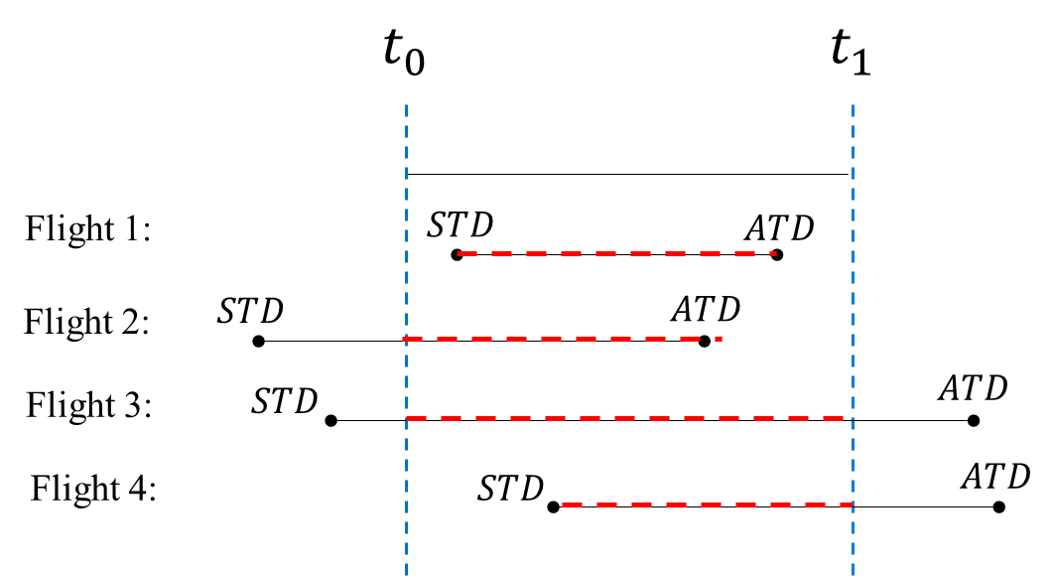
\includegraphics[width=\textwidth]{img/delay decompose.png}
    \caption{Decomposition of departure delay into time slice}
\end{figure}

In this project, the airport connections are identified based on departure delay patterns. We first construct the daily departure delay time series matrix, as illustrated in \hyperref[fig:delay matrices]{fig:delay matrices}.  Each airport has a 3 by 96 matrix. 96 represents the number of 15 min time slice of each day. Each column vector contains the 5th, 50th and 95th percentile of flight departure delay within the time slice. Each row vector is the time series of each delay statistics. The arrival delay matrices are constructed in the same way. 
\begin{figure}[thbp]
    \label{fig:delay matrices}
    \centering
    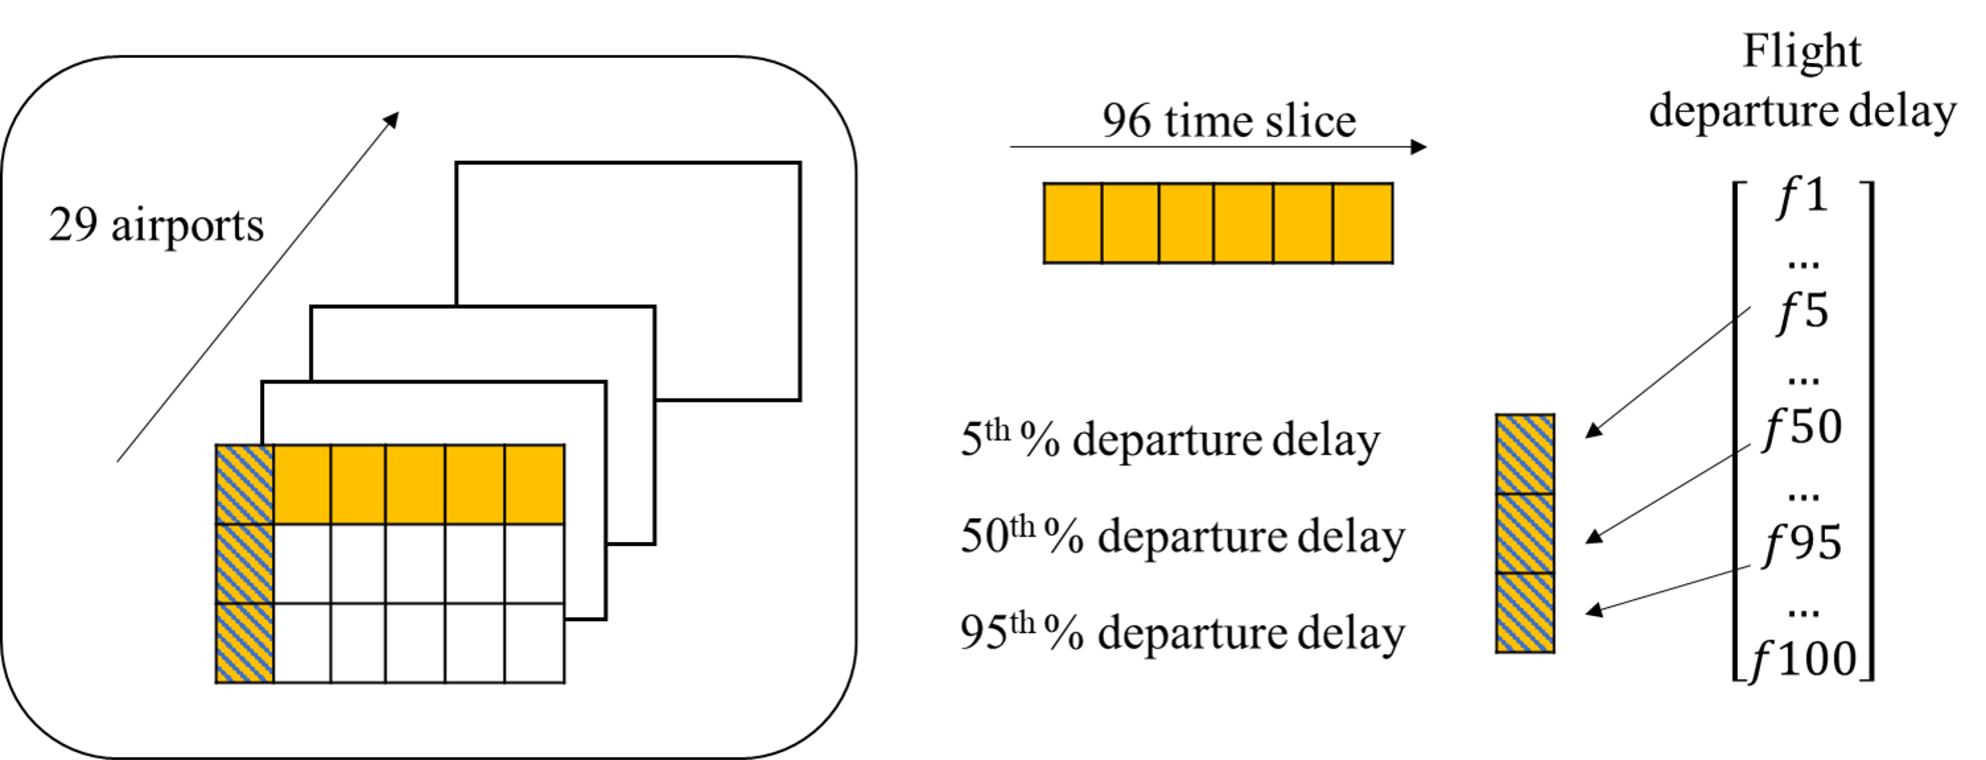
\includegraphics[width=\textwidth]{img/delay matrices.png}
    \caption{Illustration of delay matrices}
\end{figure}

Besides, we also include flight accumulation within each time step as additional features for each airport node. We construct queuing diagram for each airport, as shown in \hyperref[fig:accumulation matrix]{fig:accumulation matrix}. Then the excess accumulation at each time can be calculated by $\mathrm{E(t)}=\mathrm{S(t)}-\mathrm{A(t)}$, where $\mathrm{S(t)}$ is the scheduled cumulative departure, $\mathrm{A(t)}$ actual cumulative departure.

\begin{figure}[thbp]
    \label{fig:accumulation matrix}
    \centering
    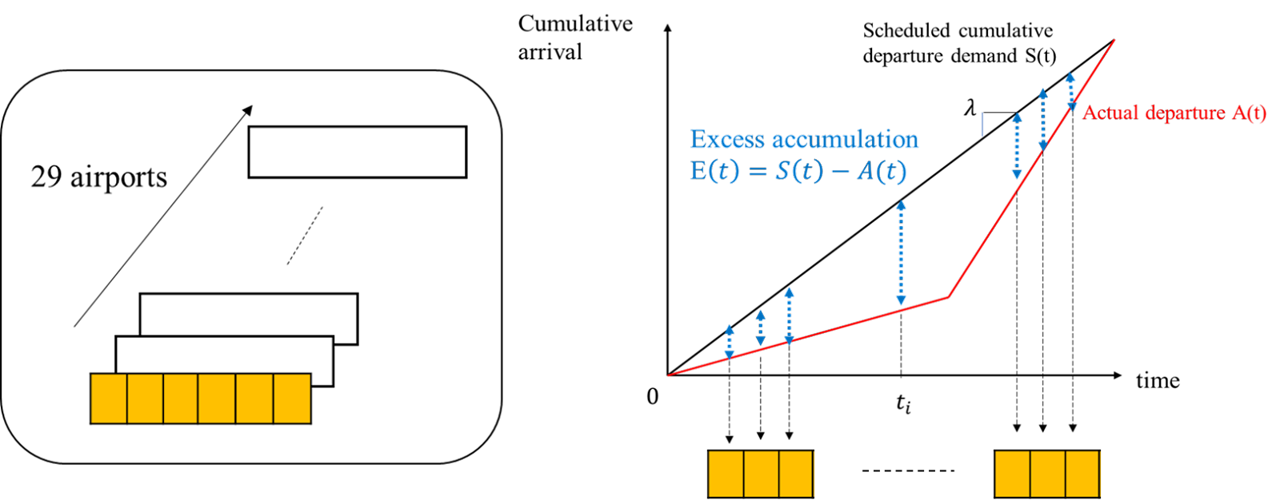
\includegraphics[width=\textwidth]{img/accumulation matrix.png}
    \caption{Illustration of accumulation matrix}
\end{figure}


%Introduction of the dataset
%Preprocess procedure
    %What features? how to generate? Why?

\section{Adaptive Deep Modularity Network (ADMoN)}

The overall framework of the adaptive deep modularity network (ADMoN) is shown in \hyperref[fig:3-1]{Figure 3.1}. As mentioned in the previous section, airport quarter delays of a single day pass a processing pipeline and generate ordered vectors. We initialize the graph structure by using a delay vector to represent the delay feature of an airport and randomly generate an adjacency matrix with each of its elements randomly sampled from a uniform distribution $U(-\frac{1}{\sqrt{n}},\frac{1}{\sqrt{n}})$. The training process of ADMoN consists of jointly optimizing two tasks: graph learning and soft clustering.

\begin{figure}[thbp]
    \label{fig:3-1}
    \centering
    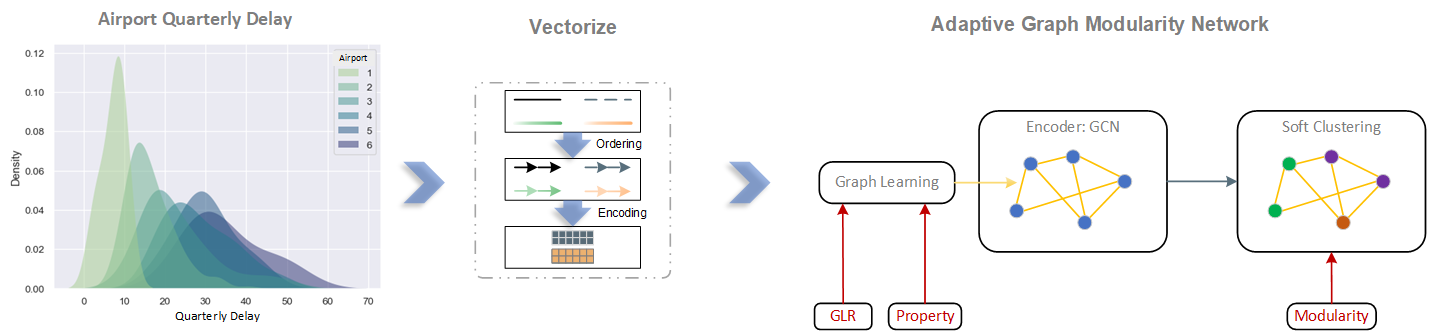
\includegraphics[width=\textwidth]{img/admon.png}
    \caption{Framework of Adaptive Deep Modularity Network}
\end{figure}

\subsection{Graph Learning}

Since the similarity of airport aggregate delay patterns are not readily available, manually construct the relationships can be sub-optimal, we implement data-driven method to extrapolate underlying relationships directly from the delay features obtained. \citet{9102726} proposed a graph learning algorithm exploiting the optimization of the adjacency matrix for both data and tasks. In our implementation, we extend its original real-value node embedding to vector embedding.

To begin with, we expect the optimal adjacency matrix to promote smoothness in graph signal, that is, edges connecting two similar nodes should be associated with higher weights than those connecting dissimilar nodes. In practice, this property can be measure by the \emph{graph Laplacian regularizer} (GLR). Define the combinatorial graph Laplacian matrix by the difference of degree matrix and adjancency matrix\citep{chung1997spectral}:
\begin{equation}
    L=D-A
\end{equation}
where the degree matrix $D$ is a diagonal matrix with its diagonal elements $d_{i,i}=\sum_{j=1}^n a_{i,j}$. Then a graph signal $\mathcal{V}\in\mathbb{R}^{n\times d}$ given on a graph $\mathcal{G}=(\mathcal{V},\tilde{A})$ is \emph{smooth} if
\begin{equation}
    \text{GLR}(\mathcal{V},\tilde{A})=\mathcal{V}^\intercal L\mathcal{V}=\mathcal{V}^\intercal\left(I-\tilde{A}\right)\mathcal{V}
\end{equation}
where $\tilde{A}$ is a normalized adjacency matrix for numerical stability of the model.
\begin{equation}
    \tilde{A}=D^{-\frac{1}{2}}AD^{-\frac{1}{2}}
\end{equation}
We integrate the GLR as a component of the total loss function weighed by $\lambda_0$ for training
\begin{equation}
    \mathcal{L}_{\text{GLR}}=\lambda_0\left\|\mathcal{V}^\intercal\left(I-\tilde{A}\right)\mathcal{V}\right\|_2^2
\end{equation}
Except for the above GLR loss, the learn-able adjacency matrix should satisfy multiple property constraints, including sparsity, symmetric, normalized, and looplessness. Similarly, we integrate them by constructing associated loss functions and assign different weights:
\begin{itemize}
    \item \textbf{Sparsity}. We promote sparse connections to enforce our model capturing only the prominent similarities. Mathematically, we use $l_1$-trick to reduce cardinality of the adjacency matrix:
    \begin{equation}
        \mathcal{L}_{\text{card}}=\lambda_1\|\tilde{A}\|_1
    \end{equation}
    \item \textbf{Symmetric}. As discussed in the previous section, we consider mutual impacts within the network and model the connections as a undirected graph. Therefore, we enforce the learned adjacency matrix to be symmetric:
    \begin{equation}
        \mathcal{L}_{\text{symmetric}}=\lambda_2\left\|\tilde{A}^\intercal-\tilde{A}\right\|_F^2
    \end{equation}
    \item \textbf{Normalized}. For stability, we enforce the learned adjacency matrix normalized:
    \begin{equation}
        \mathcal{L}_{\text{norm}}=\lambda_3\left\|\tilde{A}\textbf{1}-\textbf{1}\right\|_F^2
    \end{equation}
    where $\textbf{1}\in\mathbb{R}^n$ is a vector with all the elements equal to one.
    \item \textbf{Looplessness}. In a airport delay similarity network, it's unnecessary to link a airport with itself. Mathematically, we want the trace of the adjacency matrix to be zero:
    \begin{equation}
        \mathcal{L}_{\text{looplessness}}=\lambda_4\left|\mathbf{tr}(\tilde{A})\right|^2
    \end{equation}
\end{itemize}
With all the above settings, the graph learning process can be expressed as an optimization problem that minimize the following objective function:
\begin{equation}
    \min_{\tilde{A}} \lambda_0\left\|\mathcal{V}^\intercal\left(I-\tilde{A}\right)\mathcal{V}\right\|_2^2+\lambda_1\|\tilde{A}\|_1+\lambda_2\left\|\tilde{A}^\intercal-\tilde{A}\right\|_F^2+\lambda_3\left\|\tilde{A}\textbf{1}-\textbf{1}\right\|_F^2+\lambda_4\left|\mathbf{tr}(\tilde{A})\right|^2
\end{equation}
In this formation, we can manually tune the values of all the weights $\lambda_i,i=0,\ldots,4$ to address different property importance.

\subsection{Airport Soft Clustering}

Based on graph learning, we can directly identify latent structure of the airports by their delay patterns. Since the GLR leads to an inhomogeneous distribution of edge weights, we can infer \emph{clusters} (also known by \emph{communities} or \emph{modules}) consisting of airports with high intra-cluster weight density and low inter-cluster density. \citet{tsitsulin2020graph} proposed a Deep Modularity Network (DMoN) model which is driven by the modularity measure of clustering quality. It simultaneously learn the graph embedding and proper cluster assignments of the nodes. They use a graph convolutional neural network (GCN) \citep{https://doi.org/10.48550/arxiv.1609.02907} combined with skip connection as the kernel transformation function.
\begin{equation}
    \mathcal{K}(\mathcal{V},\tilde{A})=\text{GCN}(\mathcal{V},\tilde{A})=\tilde{A}\mathcal{V}W+\mathcal{V}W_{\text{skip}}
\end{equation}
where both $W$ and $W_{\text{skip}}$ are learn-able weight matrices that project features from high-dimensional metric space into a low-dimensional hidden space. The model is trained on an objective to maximize the spectral modularity (i.e., the measure of network division strength) and penalize assigning all the nodes into the same cluster (i.e., a collapse regularization term). The objective problem is as follows:
\begin{equation}
    \min_{W,W_{\text{skip}}}-\frac{1}{2m}\mathbf{tr}(C^\intercal AC-C^\intercal d^\intercal dC)+\frac{\sqrt{K}}{n}\left\|\sum_iC_i^\intercal\right\|_F-1: C=\text{Softmax}(\tilde{A}\mathcal{V}W+\mathcal{V}W_{\text{skip}})
\end{equation}
where $C\in\mathbb{R}^{n\times K}$ is the soft cluster results of the graph with each element $c_{ik}$ the probability of node $i$ as a member of cluster $k$, $d$ is the degree vector of all the nodes, and $m$ the number of edges. We propose to combine graph learning with DMoN to allow adaptive graph structure inference and name it Adaptive Deep Modularity Network (ADMoN).

We use "warm-up and fine-tune" strategy for training. At first, we use batches of aggregate delay features with back propagation to train the model and derive a warm-up parameter estimation. Then, we further fine-tune our model using single batch of data and obtain final adjacency matrix and cluster assignments regarding each batch of data.

\subsection{Extension: Daily Connection Identification}
\label{ch_3_3_3}

As shown in \hyperref[fig:3-2]{Figure 3.2}, if the input aggregated delay features are daily based, we can estimate the airport connections with respect to each day as adjacency matrix $A_i$. Since eigenvalues of a adjacency matrix has proven to be a useful graph features for machine learning tasks \cite{schmidt2014spectral}, we use eigenvalues of adjacency matrices to construct the node feature matrix $\mathcal{V}^\prime$ in daily connection graph.
\begin{equation}
    v_i^\prime=SP(\tilde{A})=\text{diag}(\Lambda):\tilde{A}Q=Q\Lambda, v_i^\prime\in\mathcal{V}^\prime
\end{equation}
where $\tilde{A}Q=Q\Lambda$ is the spectral decomposition of normalized adjacency matrix $\tilde{A}$. By injecting the new graph into ADMoN framework, we can identify latent connections among operational days based on airport delay connection patterns.

\begin{figure}[thbp]
    \label{fig:3-2}
    \centering
    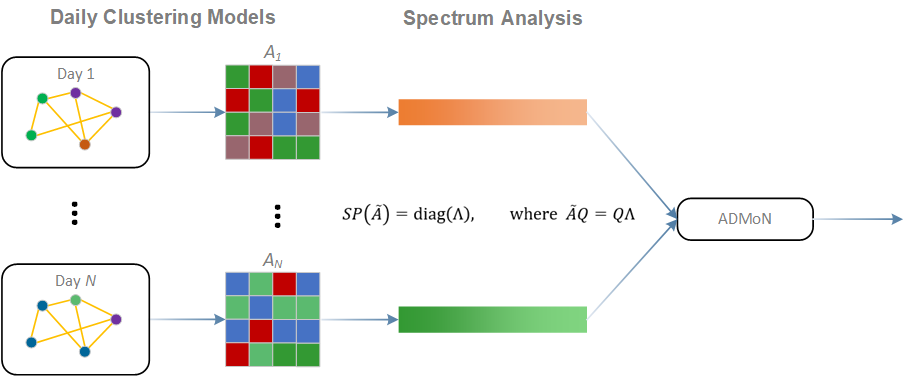
\includegraphics[width=\textwidth]{img/extension.png}
    \caption{Extension of ADMoN on inferring operational day connection}
\end{figure}

% \begin{tcolorbox}[breakable,title={An example colorbox},
% colback=founderblue!5!white,
% colframe=founderblue!75!black,
% fonttitle=\headingfont\bfseries\large]
% Your text goes here. The colors are based on Berkeley's Founder Blue.
% \tcbsubtitle[before skip=\baselineskip]%
% {You can also have subboxes}
% Don't like the colors? You can change them here (replace founderblue with the color you like), or you can change them globally in the colors section of report.tex
% \tcbsubtitle[before skip=\baselineskip]%
% {Multiple rows}
% If you like it.

% \end{tcolorbox}







\chapter{RESULTS}
\pagestyle{fancy}

In this chapter, we present the results from our proposed method. The following parts of this chapter is organized as follows: In section 4.1, we briefly introduce our experiment settings, and present the test results. Section 4.2 gives a demonstration on how we can apply our model in identifying airport delay connections based on the data from single operation day. Finally, we extend our model to investigate daily connection in section 4.3 and present the estimation.

\section{Experiments}

We assess the performance of our model in terms of both graph clustering and connection identification. 

\noindent\textbf{Baselines.} To demonstrate the power of integrating graph learning in the framework, we compare our clustering results with ones obtained using multiple predefined adjacency matrices $A_1, A_2, A_3$. Denote the great circle distance between airport $i$ and $j$ by $D_{ij}$, and the number of inter-airport flights by $N_{ij}$, we construct these adjacency matrices as follows:
\begin{equation}
    \left[A_1\right]_{ij}=\frac{1}{2}(D_{ij}+N_{ij})
\end{equation}
\begin{equation}
    \left[A_2\right]_{ij}=\frac{1}{3}(D_{ij}+2N_{ij})
\end{equation}
\begin{equation}
    \left[A_3\right]_{ij}=\frac{1}{3}(2D_{ij}+N_{ij})
\end{equation}

\noindent\textbf{Metrics.} We measure the performance of the graph clustering model using graph-level metrics: average cluster conductance \citep{yang2015defining} and graph modularity \citep{newman2006modularity}. The conductance of a cluster is defined as the fraction of total inter-cluster edge weights. We use the average level of all clusters as our performance measure and expect a low overall conductance.
\begin{equation}
    \mathcal{C}=\frac{1}{|C|}\frac{\sum_C\sum_{i\in C,j\notin C}w_{ij}}{\sum_i\sum_j w_{ij}}
\end{equation}

The graph modularity measures the sparse and dense structure of clusters compare to a random graph. A higher modularity refers to a better clustering structure.
\begin{equation}
    \mathcal{Q}=\frac{1}{C}\sum_{A_i,i\in C}\frac{1}{2m}\left(A_i-\frac{d_id_i^\intercal}{2m}\right)
\end{equation}

We fix the architecture for all clustering networks to have one hidden layer with 64 neurons in it and set the number of target clusters to 16. We use ADAM optimizer with a learning rate of 0.001 and train our model for 1000 epochs. The results are in \hyperref[tab:4-1]{Table 4.1}.

\begin{table}[thbp]
    \label{tab:4-1}
    \caption{Results of Experiments}
    \centering
    \begin{tabular}{@{}ccccccc@{}}
    \toprule
    \textbf{Features} &
      \multicolumn{2}{c}{\textbf{Dep. Delay}} &
      \multicolumn{2}{c}{\textbf{Arr. Delay}} &
      \multicolumn{2}{c}{\textbf{Dep. \& Arr. Delay}} \\ \midrule
    \textbf{Method} & $\mathcal{C}\downarrow$     & $\mathcal{Q}\uparrow$      & $\mathcal{C}\downarrow$ & $\mathcal{Q}\uparrow$      & $\mathcal{C}\downarrow$ & $\mathcal{Q}\uparrow$      \\
    GCN + $A_1$        & 0.7962          & -0.0173         & 0.6977      & -0.0133         & 0.5237      & -0.0184         \\
    GCN + $A_2$        & 0.8092          & -0.0220         & 0.7193      & -0.0216         & 0.5545      & -0.0227         \\
    GCN + $A_3$        & 0.7859          & -0.0140         & 0.6756      & -0.0077         & 0.5143      & -0.0149         \\
    \textbf{ADMoN}  & \textbf{0.2882} & \textbf{0.4110} & 0.6831      & \textbf{0.1521} & 0.5711      & \textbf{0.2554} \\ \bottomrule
    \end{tabular}
\end{table}

Judging by only the modularity, our model has a significantly better performance over those with predefined adjacency matrices, which indicates that graph learning can indeed help extrapolate the latent sparse connections based on delay features. We believe predefined adjacency matrices failed because they are not sparse enough to support graph clustering. Besides, results on dataset with only departure delay are significantly better than those with arrival delay. We believe this is due to the fact that arrival delay are to some extent affected by en-route conditions (e.g., winds, rains, etc.) which leads to variance in delay features.

\section{Airport Connection Identification}
In this section, we use a daily-level example to demonstrate how we can apply our model to identify airport delay connections based on the data from single operation day. 

\hyperref[tab:4-2]{Table 4.2} shows the airport cluster of Jul.8, 2019. To better illustrate, we draw a map to show the location of airports in \hyperref[fig:4-1]{Figure 4.1}. The color of nodes represent the cluster. The strength of connections between airports are shown in \hyperref[fig:4-2]{Figure 4.2}. We can see that clusters of airports are not purely identified by their locations. We suppose that similar airport daily delay patterns results from two aspects. First, multiple airports within a geographical region will simultaneously experience flight delays, when convective weather cover this area. Second, for other airports that are not directly affected by the weather, they will experience time lagged propagated delay by direct flights. So, results of \hyperref[fig:4-1]{Figure 4.1} indicate propagated delay by direct flights also matter in airport delay patterns. 

\begin{table}[thbp]
    \label{tab:4-2}
    \caption{Airport Clusters of Jul 8, 2019}
    \centering
    \begin{tabular}{@{}cl@{}}
    \toprule
    \textbf{Cluster No.} & \multicolumn{1}{c}{\textbf{Airports}} \\ \midrule
    \textbf{1}           & ATL, BOS, BWI, CLT, EWR, IAH, LAS     \\
    \textbf{2}           & DCA, DFW, DTW, FLL, JFK               \\
    \textbf{3} & \begin{tabular}[c]{@{}l@{}}IAD, LAX, LGA, MCO, MDW, MEM, MIA, MSP,\\ ORD, PHL, PHX, SAN, SEA, SFO, SLC, TPA\end{tabular} \\
    \textbf{4}           & DEN                                   \\ \bottomrule
    \end{tabular}
\end{table}

\begin{figure}[thbp]
    \label{fig:4-1}
    \centering
    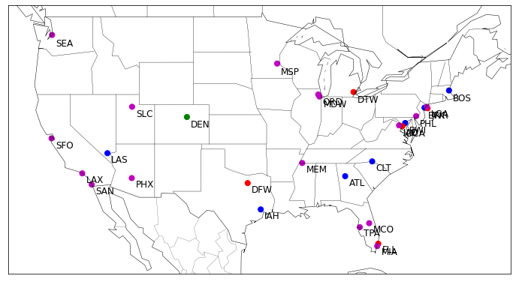
\includegraphics[width=\textwidth]{img/map of cluster.png}
    \caption{Airport clusters and locations on map (Jul.8)}
\end{figure}

\begin{figure}[t!]
    \label{fig:4-2}
    \centering
    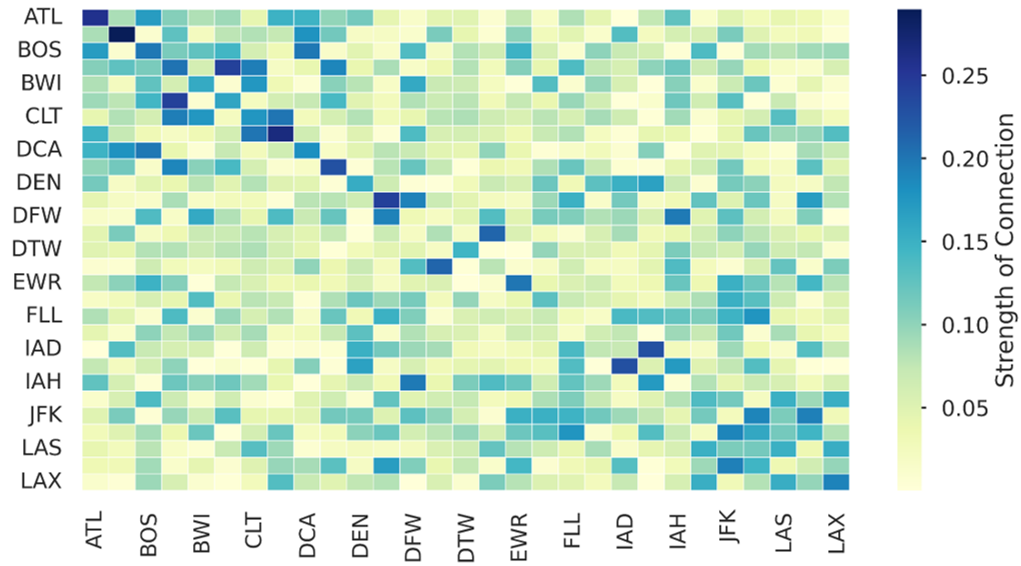
\includegraphics[width=\textwidth]{img/adjacency.png}
    \caption{Strength of Connections Between Airports (Jul.8)}
\end{figure}

We then further examine see why these airports are identified in one cluster, by looking at the departure delay excess accumulation.  \hyperref[fig:4-3]{Figure 4.3} shows the time series of departure delay excess accumulation of each airport in different clusters. In cluster 1, the airport excess accumulation is high during 0:00-04:00, and 19:00-23:59. In cluster 2, there is a relatively small accumulation during 0:00-1:00, and a high accumulation starts from the noon. In addition, in cluster 1 and 2, we can find the time series of accumulation these two clusters show some latent ‘time-lagged’ pattern, which indicates that the airports in these 2 clusters have similar patterns because of propagated delay. In each cluster, there is one airport has extreme large excess accumulation. The time series of other airports follow the pattern of this airport. We suspect that the airport with extreme large excess accumulation experienced server disruptions, and other airports are affected by the propagated flights delay. In cluster 3, the overall magnitude of excess accumulation is smaller, but the duration is longer than the other clusters. It shows that there are continual congestion at these airports during the daytime. By looking at the map, these airports are geographically close, such as TPA, MIA and MCO in the southeast coast. The continual accumulation during daytime suggests that these airports may have demand and capacity imbalance problem. Cluster 4 may be the outlier.

\begin{figure}[thbp]
    \label{fig:4-3}
    \centering
    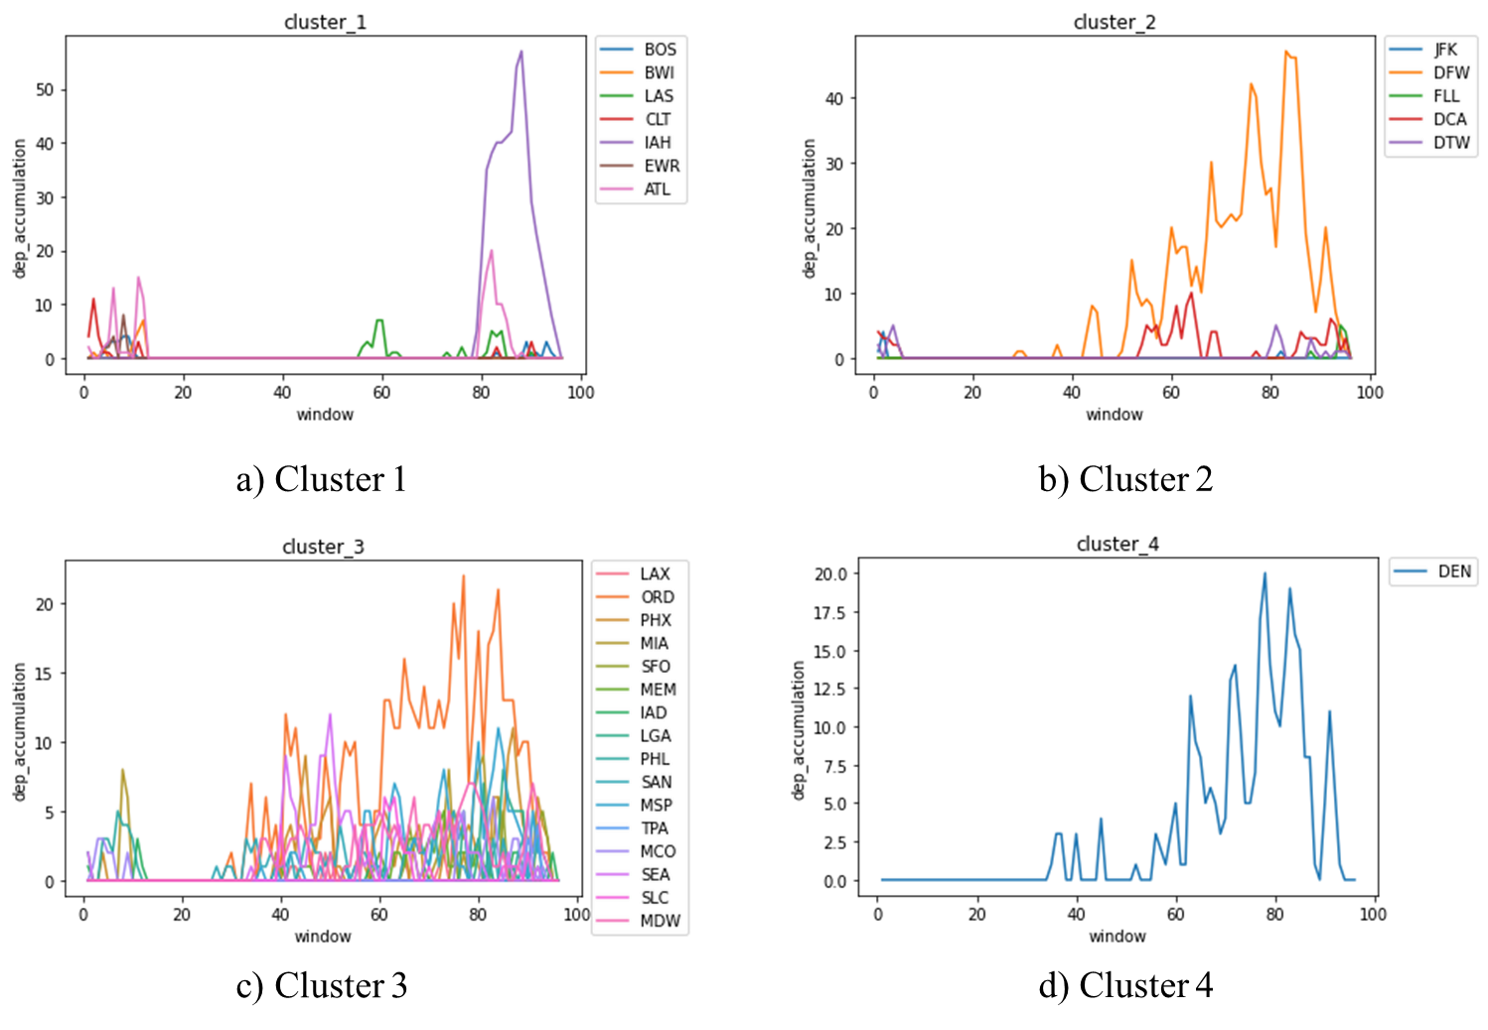
\includegraphics[width=\textwidth]{img/4 clusters.png}
    \caption{Time Series of Departure Delay Excess Accumulation (Jul.8)}
\end{figure}

We also look at the clustering results of Aug.5, 2019. The airport clusters and strength of connections are shown in \hyperref[tab:4-3]{Table 4.3} and \hyperref[fig:4-4]{Figure 4.4} respectively. Compared with \hyperref[tab:4-2]{Table 4.2} and \hyperref[fig:4-2]{Figure 4.2}, we find that some airports are in the cluster in two different days, e.g. SFO, SLC, PHX, SAN,and SEA; ATL and CLT, TPA, MCO and MIA. It motivates us to investigate the daily connextions.

\begin{table}[thbp]
    \label{tab:4-3}
    \caption{Airport Clusters of Aug 5, 2019}
    \centering
    \begin{tabular}{@{}cl@{}}
    \toprule
    \textbf{Cluster No.} & \multicolumn{1}{c}{\textbf{Airports}} \\ \midrule
    \textbf{1}           & IAD,MCO,MDW,MEM,MIA,MSP,ORD,PHL,PHX,SAN,SEA,SFO,SLC,TPA     \\
    \textbf{2}           & LAX, LGA              \\
    \textbf{3} & \begin{tabular}[c]{@{}l@{}}EWR, IAH, JFK, LAS\end{tabular} \\
    \textbf{4}           & ATL, BOS, BWI, CLT, DCA, DEN, DFW, DTW, FLL                                   \\ \bottomrule
    \end{tabular}
\end{table}

\begin{figure}[t!]
    \label{fig:4-4}
    \centering
    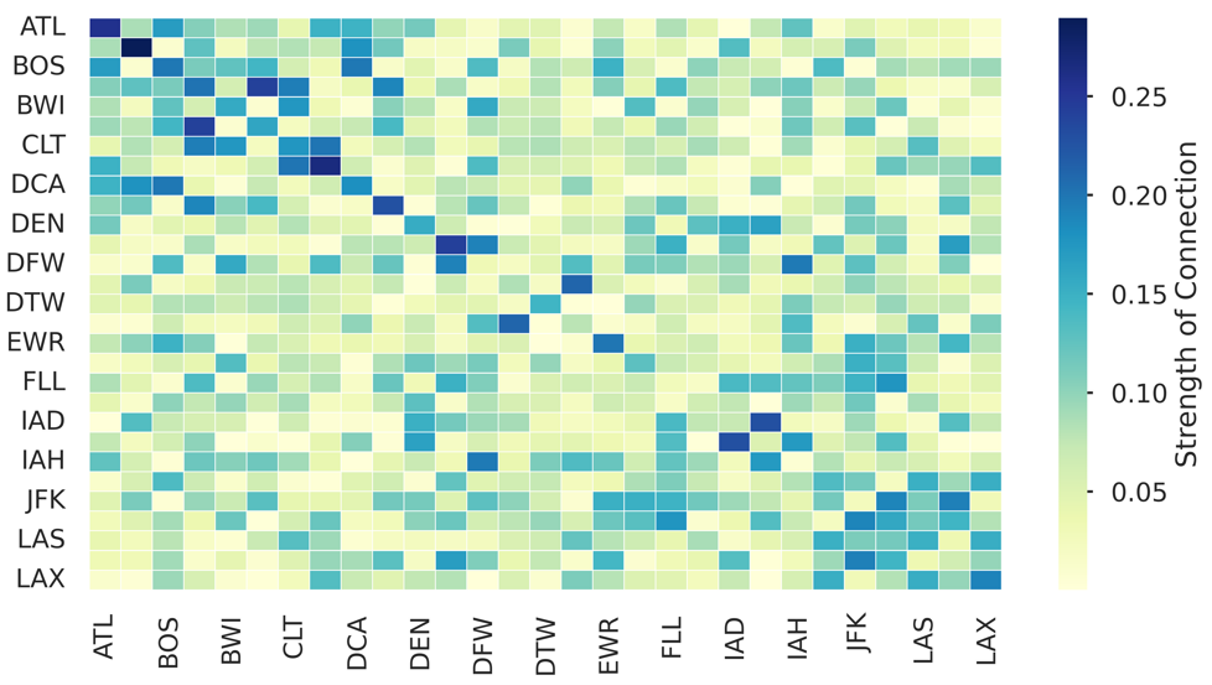
\includegraphics[width=\textwidth]{img/strength 0805.png}
    \caption{ Strength of Connections Between Airports  (Aug.5)}
\end{figure}

\section{Daily Connection Identification}

As mentioned in section 3.3.3, by using the eigenvalues of identified adjacency matrices as our new input features, our model can identify connections among operation days. 

\hyperref[fig:4-5]{Figure 4.5} shows the identification result. Overall, most of the operational days share similarities with each other, which is demonstrated by the background noises. Near the diagonal, we can see clusters at early July, mid-August, and early September. Strong connections can be see in these periods for days in the same week. But compared to the background noise, the strengths are insignificant.

\begin{figure}[thbp]
    \centering
    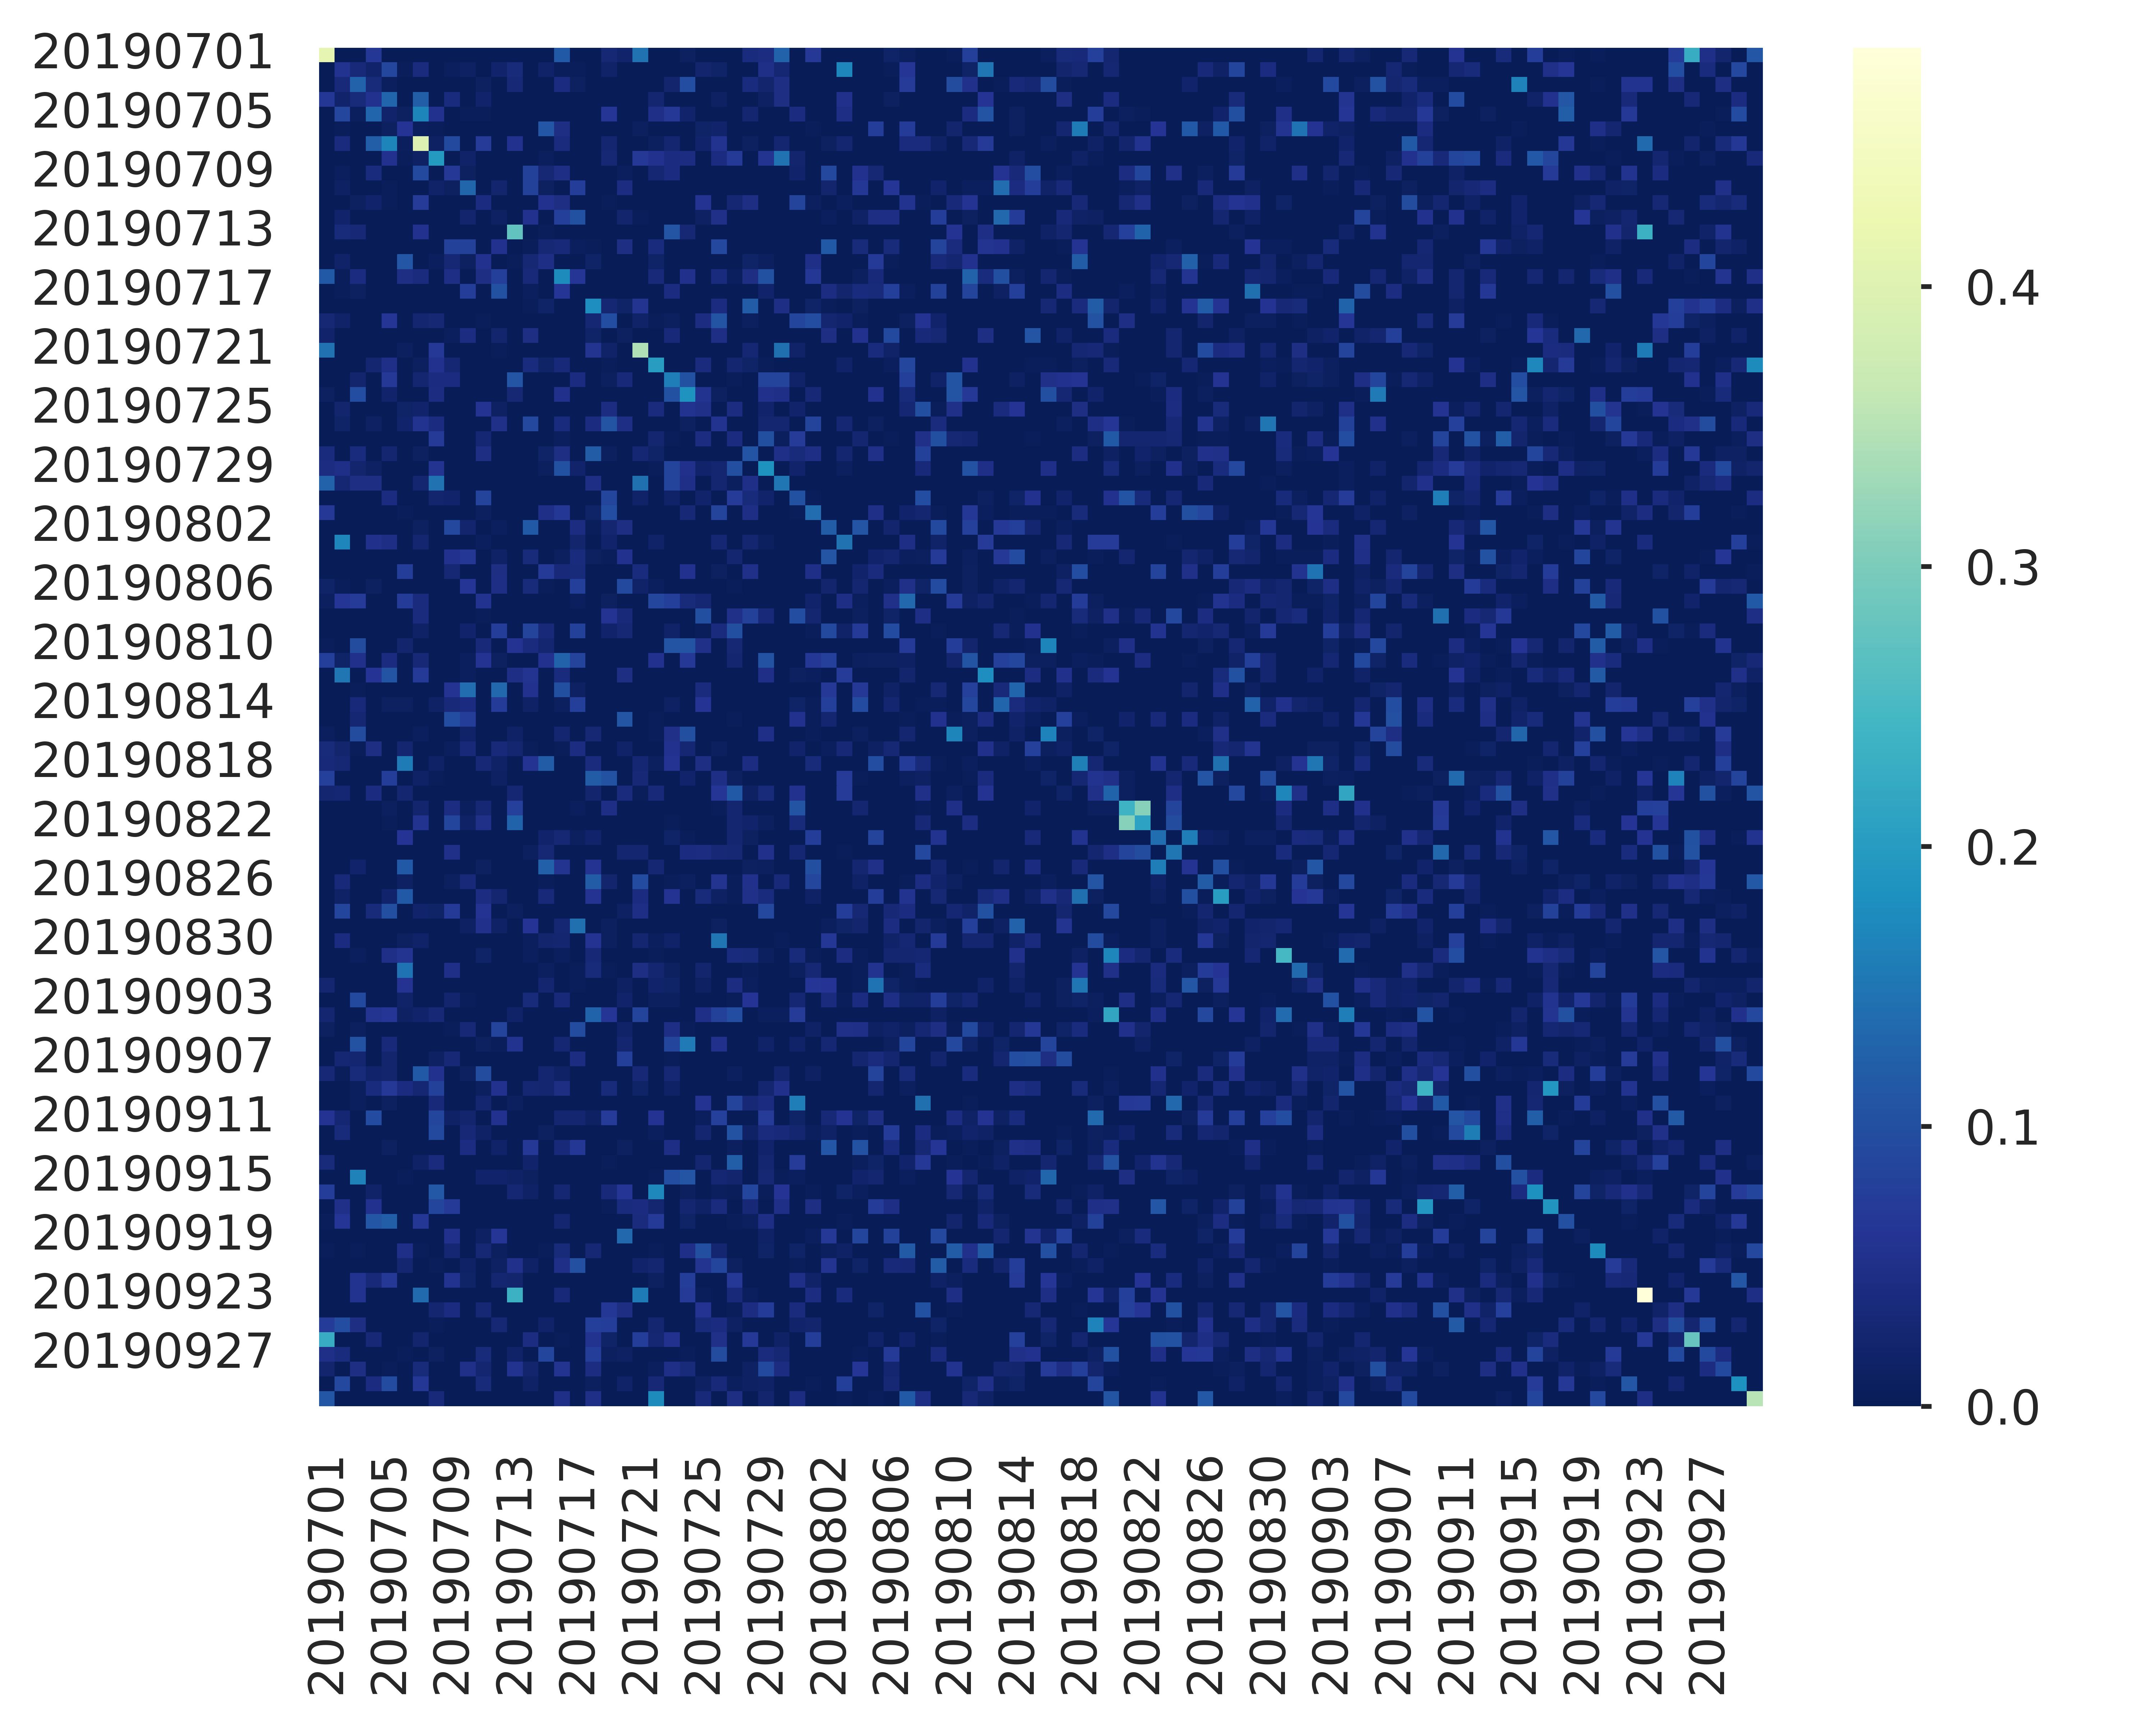
\includegraphics[width=\textwidth]{img/daily_corr.png}
    \caption{Strength of Connections Between Operation Days}
    \label{fig:4-5}
\end{figure}

% \begin{tcolorbox}[breakable,title={An example colorbox},
% colback=founderblue!5!white,
% colframe=founderblue!75!black,
% fonttitle=\headingfont\bfseries\large]
% Your text goes here. The colors are based on Berkeley's Founder Blue.
% \tcbsubtitle[before skip=\baselineskip]%
% {You can also have subboxes}
% Don't like the colors? You can change them here (replace founderblue with the color you like), or you can change them globally in the colors section of report.tex
% \tcbsubtitle[before skip=\baselineskip]%
% {Multiple rows}
% If you like it.
% \end{tcolorbox}
%include{chapter5}
\chapter{Conclusion}
\pagestyle{fancy}

In this project, we aim to identify the connections of airports in a network based on their similarities in operation delay patterns. To achieve this, we propose the Adaptive Deep Modularity Network building on existing studies. The model combines graph learning with graph clustering to learn graph structure and clustering labels simultaneously.

Compared with similar graph clustering model with a predefined adjacency matrix, our model is able to learn valid connections through data-driven pipeline and achieve a high performance judging by conductance and modularity measure. Results show that our clustering method can identify both simultaneous and time-lagged patterns similarity between airports. 

However, the limitations of our model are obvious. First, since the model is train on a data-driven pipeline, conductance and modularity performance metrics aren't intuitive for determining whether the clustering result is reasonable. Unlike some other clustering algorithms like tree-based models, our model doesn't integrate the importance measure with respect to each input feature, which can potentially be critical for interpretation. Last but not the least, since the optimization objective is complicated, training procedure can be highly sensitive to the initialization and easily converge to sub-optimal. We will address this issue in our future studies.

% We're using chapter 4 as the conclusion. If you want to have more chapters, just create more files with chapter[number].tex. Make the last one the conclusion. In order to omit the chapter number, just place an asterix before the chapter name like so:

% \textbackslash chapter*\{Conclusion\}

\chapter*{Author Statements}

The authors confirm contributions on the project as follows: \textbf{Juanwu Lu:} Conceptualization, Algorithm Design, Visualization, Writing-Reviewing and Editing. \textbf{Ying Zhou:} Conceptualization, Data Curation, Visualization, Analysis, Writing-Original draft preparation.

Special thanks to \textbf{Anton Tsitsulin} from Google Research, NYC for his generous and insightful support on realization of the graph clustering model.

% \chapter*{APPENDIX}
\pagestyle{fancy}


% This adds the conclusion to the TOC without a number
% \addcontentsline{toc}{chapter}{Conclusion}
% It is possible to add a bibliography here
% \printbibliography
\bibliographystyle{apacite}
% \bibliographystyle{plainnat}
\bibliography{reference}
% This is the back cover
% The page background is Berkeley's dark blue color


\pagecolor{berkeleyblue}
\pagestyle{empty}

% This places the back cover logo. Replace logo.png with
% your logo
\tikz[overlay, remember picture] \node at (6.5,-14) {

\includegraphics[width=0.7\textwidth]{logo.png}    
};

% This places those lines of text. Just erase Text 1, etc if you
% don't want any text

% \tikz[overlay, remember picture] \node at (6.5,-17.7) {
% \begin{tcolorbox}[colupper=white,colback=berkeleyblue,width=10cm,halign=left,boxrule=0pt]%%
%   \headingfont\Large 
%   Text 1 \\ 
%   Text 2 \\ 
%   Text 3
% \end{tcolorbox}
% };



% This code creates decorative `colorboxes' for text
% illustrations and the like. Just uncomment it and place
% it in a chapter

% \begin{tcolorbox}[breakable,title={An example colorbox},
% colback=founderblue!5!white,
% colframe=founderblue!75!black,
% fonttitle=\headingfont\bfseries\large]
% Your text goes here.
% \tcbsubtitle[before skip=\baselineskip]%
% {You can also have subboxes}
% with extra content
% \tcbsubtitle[before skip=\baselineskip]%
% {Multiple rows}
% If you like it.
% \end{tcolorbox}


% This code creates a decorative text box. 
% Just uncomment it and place
% it in a chapter

% \begin{mybox}{Hello World!}

% This is the mybox environment.

% However, the problem with mybox is that they cannot break across pages :( So, they have to be pretty short. Otherwise use the colorbox

% \end{mybox}





\end{document}

